\documentclass{report}


\usepackage[T1]{fontenc}
\usepackage[utf8]{inputenc}
\usepackage{amsmath}


\usepackage{enumerate}
\usepackage{trfsigns}
\usepackage{graphicx}
\usepackage{fancyhdr}
\usepackage{lettrine}
\usepackage{hyperref}
\usepackage{subcaption}
\usepackage{tikz}
\usepackage{cite}
\usepackage{listings}
\usepackage[nottoc, numbib]{tocbibind}
\usepackage[ngerman]{babel}
\usepackage[Sonny]{fncychap}
\usepackage{trfsigns}
\usepackage{parskip}
\usepackage{microtype}
\usepackage{gensymb}


\usetikzlibrary{shapes}
\usetikzlibrary{arrows}
\usetikzlibrary{arrows.meta,topaths}
\usetikzlibrary{bending}
\usetikzlibrary{calc}
\title{Elektrotechnik 1 Praktikum 1}


\usepackage[
	includehead,
	headheight = 17mm,
	footskip = \dimexpr\headsep+\ht\strutbox\relax,
	tmargin = 0mm,
	bmargin = \dimexpr17mm+2\ht\strutbox\relax,
]{geometry}

\usepackage{anyfontsize}
\usepackage{float}
\usepackage{xcolor}

\definecolor{DarkGreenBlue}{HTML}{264653}
\definecolor{LightGreenBlue}{HTML}{2A9D8F}
\definecolor{LightOrange}{HTML}{E9C46A}
\definecolor{DarkOrange}{HTML}{F4A261}
\definecolor{RedOrange}{HTML}{E76F51}
\definecolor{BrightRed}{HTML}{D62828}
\definecolor{DeepBlue}{HTML}{003049}

\lstdefinestyle{code}{
	backgroundcolor=\color{backcolour},
	commentstyle=\color{codegreen},
	keywordstyle=\color{magenta},
	numberstyle=\tiny\color{codegray},
	stringstyle=\color{codepurple},
	basicstyle=\ttfamily\footnotesize,
	breakatwhitespace=false,
	breaklines=true,
	captionpos=b,
	keepspaces=true,
	numbers=left,
	numbersep=5pt,
	showspaces=false,
	showstringspaces=false,
	showtabs=false,
	tabsize=2
}

\definecolor{codegreen}{rgb}{0,0.6,0}
\definecolor{codegray}{rgb}{0.5,0.5,0.5}
\definecolor{codepurple}{rgb}{0.502,0.502,0.0}
\definecolor{backcolour}{rgb}{0.95,0.95,0.95}

\pagestyle{fancy}
\fancyhead[L]{\leftmark}
\fancyhead[R]{\today}
\fancyfoot[L]{}
\fancyfoot[C]{\thepage}
\fancyfoot[R]{\includegraphics[]{./assets/img/LogoTI.png}}
\renewcommand\headrulewidth{0.5pt}


\begin{document}


\thispagestyle{empty}
\begin{tikzpicture}[overlay,remember picture]
	\thispagestyle{empty}
	\fill[black!2] (current page.south west) rectangle (current page.north east);

	\begin{scope}[transform canvas ={rotate around ={45:($(current page.north west)+(-.5,-6)$)}}]

		\shade[rounded corners=18pt, left color=DarkGreenBlue, right color=LightGreenBlue] ($(current page.north west)+(-.5,-6)$) rectangle ++(9,1.5);

	\end{scope}

	\begin{scope}[transform canvas ={rotate around ={45:($(current page.north west)+(.5,-10)$)}}]

		\shade[rounded corners=18pt, left color=LightOrange,right color=DarkOrange] ($(current page.north west)+(0.5,-10)$) rectangle ++(15,1.5);

	\end{scope}

	\begin{scope}[transform canvas ={rotate around ={45:($(current page.north west)+(0.5,-10)$)}}]

		\shade[rounded corners=8pt, right color=DarkOrange, left color=LightOrange] ($(current page.north west)+(1.5,-9.55)$) rectangle ++(7,.6);

	\end{scope}

	\begin{scope}[transform canvas ={rotate around ={45:($(current page.north)+(-1.5,-3)$)}}]

		\shade[rounded corners=12pt, left color=DeepBlue!80, right color=DeepBlue!60] ($(current page.north)+(-1.5,-3)$) rectangle ++(9,0.8);

	\end{scope}

	\begin{scope}[transform canvas ={rotate around ={45:($(current page.north)+(-3,-8)$)}}]

		\shade[rounded corners=28pt, left color=BrightRed, right color=BrightRed!80] ($(current page.north)+(-3,-8)$) rectangle ++(15,1.8);

	\end{scope}

	\begin{scope}[transform canvas ={rotate around ={45:($(current page.north west)+(4,-15.5)$)}}]

		\shade[rounded corners=25pt, left color=RedOrange, right color=DarkOrange] ($(current page.north west)+(4,-15.5)$) rectangle ++(30,1.8);

	\end{scope}

	\begin{scope}[transform canvas ={rotate around ={45:($(current page.north west)+(13,-10)$)}},]

		\shade[rounded corners=22pt, left color=DeepBlue,right color=DarkGreenBlue] ($(current page.north west)+(13,-10)$) rectangle ++(15,1.5);

	\end{scope}

	\begin{scope}[transform canvas ={rotate around ={45:($(current page.north west)+(18,-8)$)}},]

		\shade[rounded corners=8pt, left color=DarkOrange] ($(current page.north west)+(18,-8)$) rectangle ++(15,0.6);

	\end{scope}

	\begin{scope}[transform canvas ={rotate around ={45:($(current page.north west)+(19,-5.65)$)}},]

		\shade[rounded corners=12pt, left color=RedOrange] ($(current page.north west)+(19,-5.65)$) rectangle ++(15,0.8);

	\end{scope}

	\begin{scope}[transform canvas ={rotate around ={45:($(current page.north west)+(20,-9)$)}}]

		\shade[rounded corners=20pt, left color=BrightRed, right color=BrightRed!80] ($(current page.north west)+(20,-9)$) rectangle ++(14,1.2);

	\end{scope}

	\draw[ultra thick,gray] ($(current page.center)+(5,2)$) -- ++(0,-3cm) node[midway,left=0.25cm,text width=5cm,align=right,black!75]{{\fontsize{25}{30} \selectfont \includegraphics[width=\textwidth]{./assets/img/LogoTI.png}}} node[midway,right=0.25cm,text width=6cm,align=left,orange]{{\fontsize{70}{86} \selectfont 2023}};

	\node at ($(current page.center)+(0,-4)$) {{\fontsize{40}{72} \selectfont Reglersynthese - Digitale Regler}};

	\node[text width=8cm,align=center] at ($(current page.center)+(0,-6.5)$) {{\fontsize{16}{20} \selectfont \textcolor{orange}{ \bf \today}} \\[3pt] Domenic Heidemann 2432491\\[3pt] Emily Antosch 2519935 \\[3pt] Kevin Petri 2575357\\[3pt]};

\end{tikzpicture}

\newpage

\tableofcontents

\listoffigures
\newpage
\chapter{Regelung mit quasi-stetigen und zeitdiskreten Reglern}
\section{Vorbereitung}
% Emily
\subsection{Diskretisierung von I-Reglern}
\label{sec:diskr-von-i}


Um im Verlaufe des Praktikums verschiedene Regler und ihre Eigenschaften beim Regeln der Beleuchtungsstärke beobachten zu können, wird exemplarisch der I-Regler mithilfe der linken Rechteckregel diskretisiert. Die Abtastzeit $T_A$ beträgt $T_A = 0.001\mathrm{s}$. Die Strecke wird durch die Übertragungsfunktion $G(s)$ beschrieben. Diese lautet:
$$G_{R}(s) = \frac{K_{I}}{s}$$

Für $s$ setzen wir nun $\frac{1-\frac{1}{z}}{T_{a}}$:

$$G_{R}(z) = \frac{K_{I}T_{a}}{1-\frac{1}{z}}$$

Mit ein wenig Umstellen und Zusammenfassen der Terme erhalten wir zum Schluss:

$$G_{R}(z) = \frac{K_{I}T_{a}z}{z-1}$$

\subsection{Koeffizienten für I- und PI-Regler bestimmen}
\label{sec:koeffizienten-fur-i}

Mithilfe des Berichts können nun die Koeffizienten der digitalen I- und PI-Regler bestimmt werden. Für beide Regler gilt $a_{0} = 1$ und $a_{1} = -1$. Für den I-Regler gilt:

\begin{align}
	\label{eq:1}
	b_{0} & = T_{a}K_{I} \\
	b_{1} & = 0
\end{align}

Und für den PI-Regler gilt:

\begin{align}
	\label{eq:2}
	b_{0} & = K_{P} \cdot (1 + \frac{T_{a}}{T_{n}}) \\
	b_{1} & = -K_{P}
\end{align}

Nun soll jeweils für $T_{a} = 1ms$ und $T_{a} = 20ms$ die entsprechenden Koeffizienten berechnet werden. Es folgt:

\begin{table}[!ht]
	\centering
	\begin{tabular}{|l|l|l|l|}
		\hline
		Regler                     & Abtastzeit $T_{a}$ & $b_{0}$    & $b_{1}$ \\
		\hline
		\multirow{2}{*}{PI-Regler} & $1ms$              & $3,9466$   & $-3,94$ \\
		\cline{2-4}
		                           & $20ms$             & $4,071333$ & $-3,94$ \\
		\hline
		\multirow{2}{*}{I-Regler}  & $1ms$              & $0,00121$  & $0$     \\
		\cline{2-4}
		                           & $20ms$             & $0,0242$   & $0$     \\
		\hline
	\end{tabular}
	\caption{Koeffizienten für die digitalen I- und PI-Regler}
	\label{tab:koeIPI}
\end{table}


\subsection{Simulation der digitalen Regler}
\label{sec:simul-der-digit}

Mithilfe von Simulink können nun im Vorfeld die Regler bereits auf ihre Plausibilität hin überprüft werden. Dazu wird die Strecke mit Übertragungsfunktionsgliedern aufgebaut und die Regler jeweils mit zeitdiskreten Blöcken simuliert. Als globale Abtastrate wird $T_{a_{\mathrm{global}}} = 1ms$ gewählt. Im Block selbst kann dann eine lokale Abtastrate von jeweils $T_{a} = 20ms$ eingestellt werden. Das Ergebnis ist in~\ref{fig:sim-i-pi} zu sehen.

\begin{figure}[!ht]
	\centering
	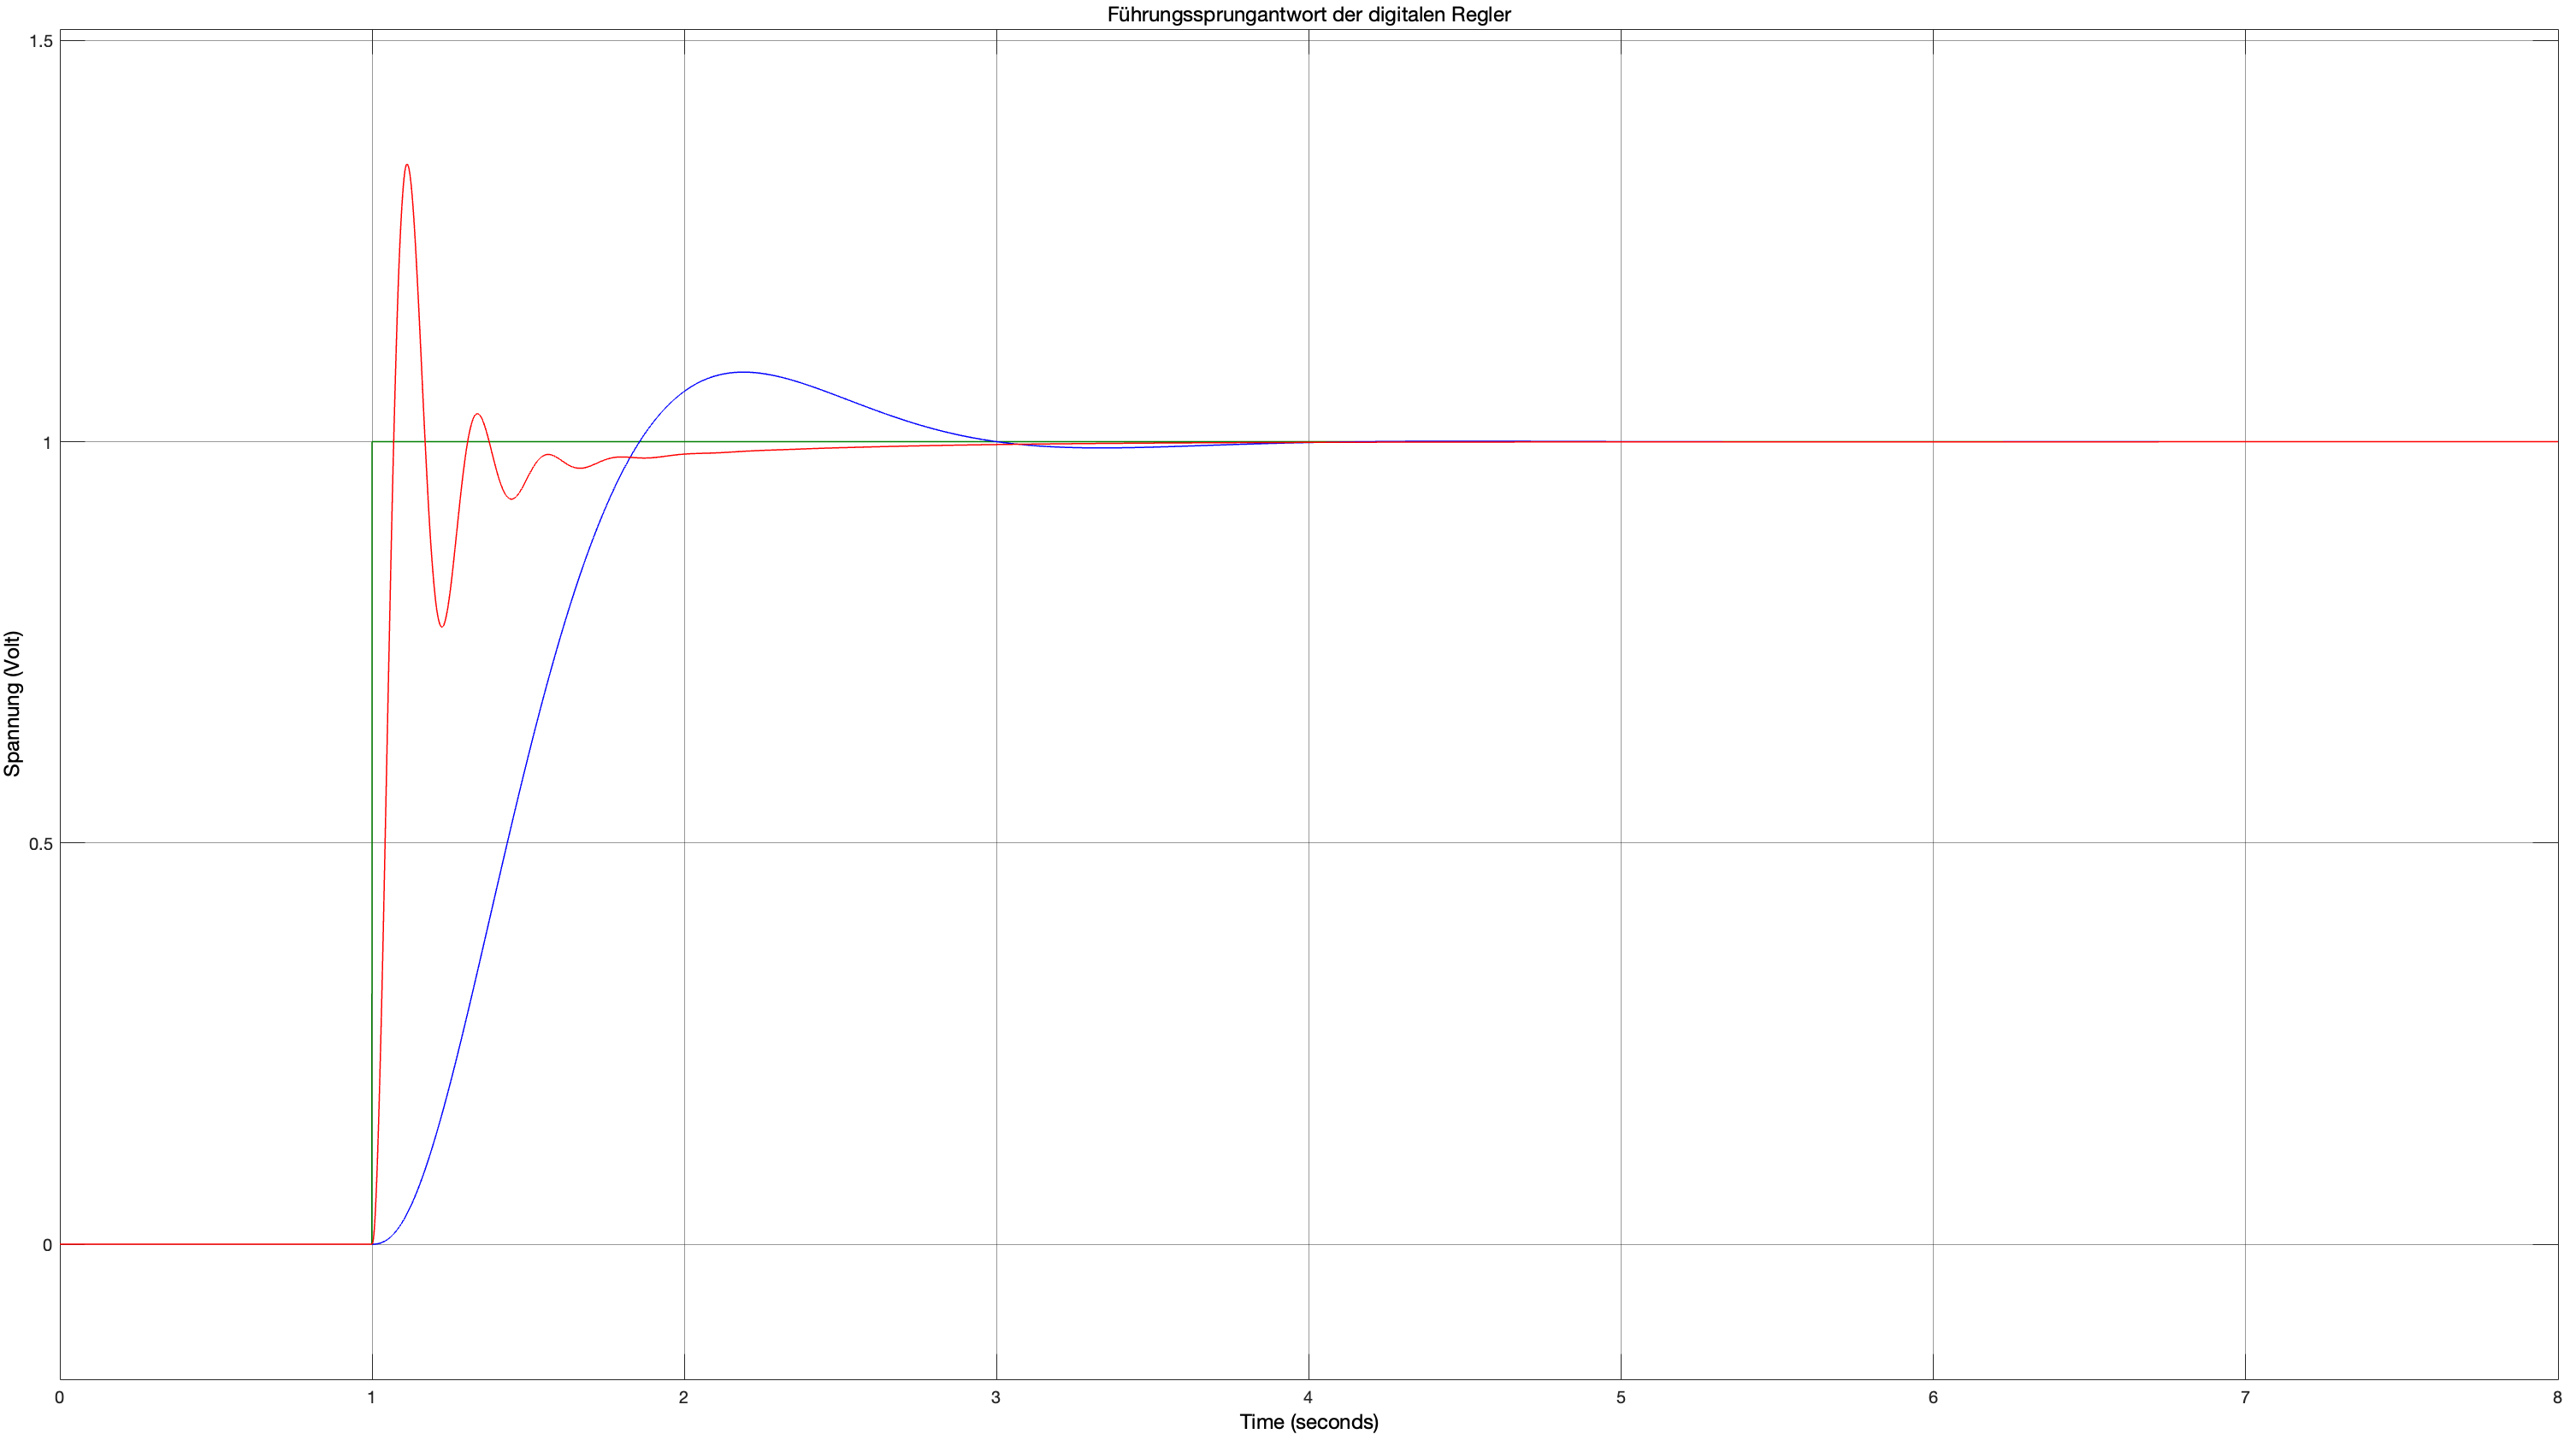
\includegraphics[width=\textwidth]{./assets/img/sim_i_pi.png}
	\caption{Die Simulation der Reglertypen bei $T_a = 20ms$ }
	\label{fig:sim-i-pi}
\end{figure}


% Wahrscheinlich noch die Plots aus der Simulation einfügen, dann kann man die auch bei den Messungen referenzieren

\section{Messungen}
\textmd{Im Labor werden die Führungssprungantworten der vorherigen Gruppe bezüglich P-, I- und PI-Regler sowie die Arbeitspunktaufschaltung repliziert und dann die in der Vorbereitung ausgelegten zeitdiskreten Regler getestet.}


\subsection{I-Regler}
\textmd{Beginnend mit dem I-Regler wird die Anlage in Betrieb genommen und eine Führungssprungantwort aufgenommen:}
\begin{figure}[H]
	\centering
	\includegraphics[scale=0.4]{Bilder/M3.1.png}
	\caption{I-Regler}
	\label{fig:M3.1.png}
\end{figure}
\textmd{Auffällig ist eine leichte stationäre Ungenauigkeit beim Führungsgröße 2,2.}


\subsection{PI-Regler}
\textmd{Der I-Regler wird in Simulink durch den PI-Regler ersetzt und die Führungssprungantwort wiederholt:}
\begin{figure}[H]
	\centering
	\includegraphics[scale=0.4]{Bilder/M3.2.png}
	\caption{PI-Regler}
	\label{fig:M3.2.png}
\end{figure}
\textmd{Der PI-Regler ähnelt sehr stark sowohl Simulation als auch den Vorergebnissen, mit Überschwinger und vergleichsweise schnellem Erreichen der Führungsgröße.}

\subsection{P-Regler}
\textmd{Zuletzt wird noch die Führungssprungantwort des P-Reglers repliziert:}
\begin{figure}[H]
	\centering
	\includegraphics[scale=0.4]{Bilder/M3.3.png}
	\caption{P-Regler}
	\label{fig:M3.3.png}
\end{figure}
\textmd{Wie erwartet ist der P-Regler ohne sonstige Anpassungen deutlich stationär ungenau und entspricht damit im Verlauf sowohl Simulation als auch den Ergebnissen der Vorgruppe.}

\subsection{Anpassung der Sollwertspannungen}

\begin{figure}[H]
	\centering
	\includegraphics[scale=0.4]{Bilder/M3.4.png}
	\caption{P-Regler mit Anpassung der Sollwertspannungen}
	\label{fig:M3.4.png}
\end{figure}


\subsection{Arbeitspunktaufschaltung}

Um die stationäre Genauigkeit des P-Reglers zu verbessern, wird eine Arbeitspunktaufschaltung durchgeführt. Dazu wird am Ausgang des Reglers eine Aufschaltung der Steuerspannung $U_{StA} = 3,43V$ vorgenommen. Diese Aufschaltung der Spannungen verschiebt den Nullpunkt auf den gewählten Arbeitspunkt von $\alpha = 90°$. Während in den ersten Teilen des Versuchs eine Aufschaltung der Spannung mittels einer OP-Schaltung geschehen ist, wird hier einfach ein Addierer in das Simulink-Bild eingebaut, welcher die Spannung $U_{StA}$ auf die Steuerspannung $U_{St}$ addiert. Die Führungssprungantwort ist in Abbildung \ref{fig:M3.5.png} zu sehen. Es ist deutlich zu erkennen, dass die stationäre Genauigkeit des P-Reglers durch die Aufschaltung der Spannung verbessert wurde, da der P-Regler nun um den Arbeitspunkt herum regelt und nicht von einer arbiträren Spannung aus.


\begin{figure}[!ht]
	\centering
	\includegraphics[scale=0.4]{Bilder/M3.5.png}
	\caption{P-Regler mit Arbeitspunktaufschaltung}
	\label{fig:M3.5.png}
\end{figure}

\subsection{Zeitdiskrete Regler, Abtastzeit $T_a=1\,ms$}
Nach der Zeitdiskretisierung des I-Reglers und der Einbindung in Simulink wird die Führungssprungantwort aufgenommen. Die Abtastzeit beträgt $T_a=1\,ms$. Es ist deutlich zu  erkennen, dass der zeitdiskrete I-Regler ziemlich nahe an dem Ergebnis des quasi-stetigen I-Reglers ist. Der Graph ist glatt und weist kaum Artefakte auf.

\begin{figure}[!arbit            \centering
	\includegraphics[scale=0.4]{Bilder/M3.6 I-Regler.png}
	\caption{Zeitdiskreter I-Regler, $T_a=1\,ms$}
	\label{fig:m36iregler}
\end{figure}

Auch der zeitdiskrete PI-Regler bei einer Abtastzeit von $T_a=1\,ms$ ist dem quasi-stetigen PI-Regler sehr ähnlich. Der Graph ist glatt und weist kaum Artefakte auf.

\begin{figure}[!ht]
	\centering
	\includegraphics[scale=0.4]{Bilder/M3.6 PI-Regler.png}
	\caption{Zeitdiskreter PI-Regler, $T_a=1\,ms$}
	\label{fig:m36piregler}
\end{figure}


\subsection{Zeitdiskrete Regler, Abtastzeit $T_a=20\,ms$}

Nach dem Erhöhen der Abtastzeit auf $T_{a} = 20\,ms$ ist deutlich zu erkennen, dass der zeitdiskrete I-Regler ein deutliches Zittern aufweist. Das ist durch die geringere Abtastrate der Messwerte zu erklären.

\begin{figure}[!ht]
	\centering
	\includegraphics[scale=0.4]{Bilder/M3.7 I-Regler.png}
	\caption{Zeitdiskreter I-Regler, $T_a=20\,ms$}
	\label{fig:M3.7 I-Regler png}
\end{figure}

Der PI-Regler bei einer Abtastzeit von $T_a=20\,ms$ weist ebenfalls ein deutliches Zittern auf. In beiden Fällen stört dieser Sachverhalt allerdings weder die Fähigkeit, die Strecke zu regeln, noch verschlechtert sie maßgeblich Gütefaktoren wie die stationäre Genauigkeit.

\begin{figure}[!ht]
	\centering
	\includegraphics[scale=0.4]{Bilder/M3.7 PI-Regler.png}
	\caption{Zeitdiskreter PI-Regler, $T_a=20\,ms$}
	\label{fig:M3.7 PI-Regler png}
\end{figure}



\newpage

\section{Auswertung}

\textmd{Nach der Diskussion der Messergebnisse werden nun noch basierend auf der Arbeitspunktaufschaltungsmessung der Regelfaktor r berechnet und anhand der Messungen zu den zeitdiskreten Reglern der Einfluss der Abtastzeit untersucht.}% Oder so.

\subsection{Regelfaktor r}
\textmd{Der Regelfakotr r gibt an um wie viel sich die Führungsgröße zur Regelgröße abweicht.}
\begin{figure}[H]
	\centering
	\includegraphics[scale=0.4]{Bilder/M3.5 mit daten Punkten.png}
	\caption{Datenpunkte zur Regelfaktorermittlung}
	\label{fig:M3.5 mit daten Punkten png}
\end{figure}
\textmd{Mit hilfe der Daten Punkten aus der Abbildung \ref{fig:M3.5 mit daten Punkten png} wird der Regefaktor r wie folgt bestimmt}

% NOTE: Ich hab hier mal die Berechnung geändert, weil das vorher ein bisschen viel war. Nach meinem Verständnis ist das auch das Verhältnis der Differenzen von Führungssprung oben und und unten und der Abstand zwischen oben und unten jeweils.
\begin{align*}
	r & = \frac{\Delta \mathrm{geregelt}}{\Delta \mathrm{ungeregelt}}=\frac{(3,1-2,85123)+(1,45226-1,4)}{3,1-1,4} \\
	r & = 0,19998
\end{align*}


\subsection{Einfluss der Abtastzeit}

\end{document}
